\documentclass[english]{scrartcl}

\usepackage{a4wide}
\usepackage[T1]{fontenc}
\usepackage[latin1]{inputenc}
\usepackage{epsfig}
\usepackage{listings}

\lstset{% set listing parameters
	language=sh,		% code in shell
	breaklines=true,	%
	linewidth=\textwidth,	% base line width for listings
	showstringspaces=false,	% do not show spaces in strings
	showspaces=false,	% do not show spaces in the code
	basicstyle=\small,	% text size
	commentstyle=\texttt,	% comment in typewriter style
	framextopmargin=10pt,	% top margin frame
	framexbottommargin=10pt,% bottom margin frame
	frame=tb}		% frame at top and bottom of the code


\IfFileExists{url.sty}{\usepackage{url}}
                       {\newcommand{\url}{\texttt}}

% \makeatletter

%%%%%%%%%%%%%%%%%%%%%%%%%%%%%% LyX specific LaTeX commands.
\newcommand{\noun}[1]{\textsc{#1}}

\usepackage{babel}
% \makeatother
\begin{document}

\title{A Tiny Queuing System for \noun{Blast} Servers}


\author{\noun{Colas Schretter}\footnote{cschrett@ulb.ac.be} and \noun{Laurent Gatto}\footnote{lgatto@ulb.ac.be}}

\maketitle

%%%%%%%%%%%%%%%%%%%%%%%%%%%%%%%%%%%%%%%%%%%%%%%%%%%%%%%%%%%%%%%%%%%%%%%%%%%%%%%%%%%%%%%%%%%%%%%%%%%%%
%%%%%%%%%%%%%%%%%%%%%%%%%%%%%%%%%%%%%%%%%%%%%%%%%%%%%%%%%%%%%%%%%%%%%%%%%%%%%%%%%%%%%%%%%%%%%%%%%%%%%

\section*{Introduction}

With the aim to assists researchers for a rapid and automated oligonucleotide design, we developed an online multi-users bioinformatic application. People could submit several design jobs and order results through a web portal. Therefore, several submission could occur independently in the same time. 

Some design jobs need to launch a similarity search across a nucleotide \noun{Blast} database. This IO-bound process requires to limit the number of such queries executed in parallel on the \noun{Blast} server. Therefore we setup a queuing system to ensure that, at any time, the executed jobs do not require more than the available IO resources.

Existing queuing systems like PBS or OpenPBS (\url{http://pbs.mrj.com}), Maui (\url{http://www.clusterresources.com}) or Sun Grid Engine (\url{http://gridengine.sunsource.net}) could be installed to solve these requirements.

However, we developed a set of shell scripts that work together to add lightweight queuing abilities to any UNIX systems. The features of our solution are:

\begin{itemize}
	\item it only rely on shell scripts and the crontab service
	\item it uses e-mail notification
	\item it can be set up with users privileges only
	\item it supports distant execution of jobs through SSH
	\item it is easily to install, use and configure
\end{itemize}

The set of scripts of a real-case application are given and commented. This document should help anyone to adapt those scripts and extend the system for further requirements.

%%%%%%%%%%%%%%%%%%%%%%%%%%%%%%%%%%%%%%%%%%%%%%%%%%%%%%%%%%%%%%%%%%%%%%%%%%%%%%%%%%%%%%%%%%%%%%%%%%%%%
%%%%%%%%%%%%%%%%%%%%%%%%%%%%%%%%%%%%%%%%%%%%%%%%%%%%%%%%%%%%%%%%%%%%%%%%%%%%%%%%%%%%%%%%%%%%%%%%%%%%%

\section*{Framework}

In the following sections, we describe each functionality by providing the scripts end their dependencies. First, we describe how any user could submit a job to the system. Then, we explain how we implemented the queuing mechanism. We setup an active system loop that watches for the presence of new job requests and a locking mechanism to limit resources usages. 


We have chosen to distribute the computation charge among several independent and dedicated servers. In our application, a web server is the entry-point to job submissions, it manages the queues and results directories. In order to ensures interactive performances to any visitor of our web server, we wanted to reserve the resources of this server exclusively for dynamic web page generation. It will also be in charge of the mailing capabilities. Resource-consuming tasks are not allowed to run on the web server. Therefore, executables are launched on a third party application server, parameters and results are stored on the web server.

\bigskip

\begin{center}
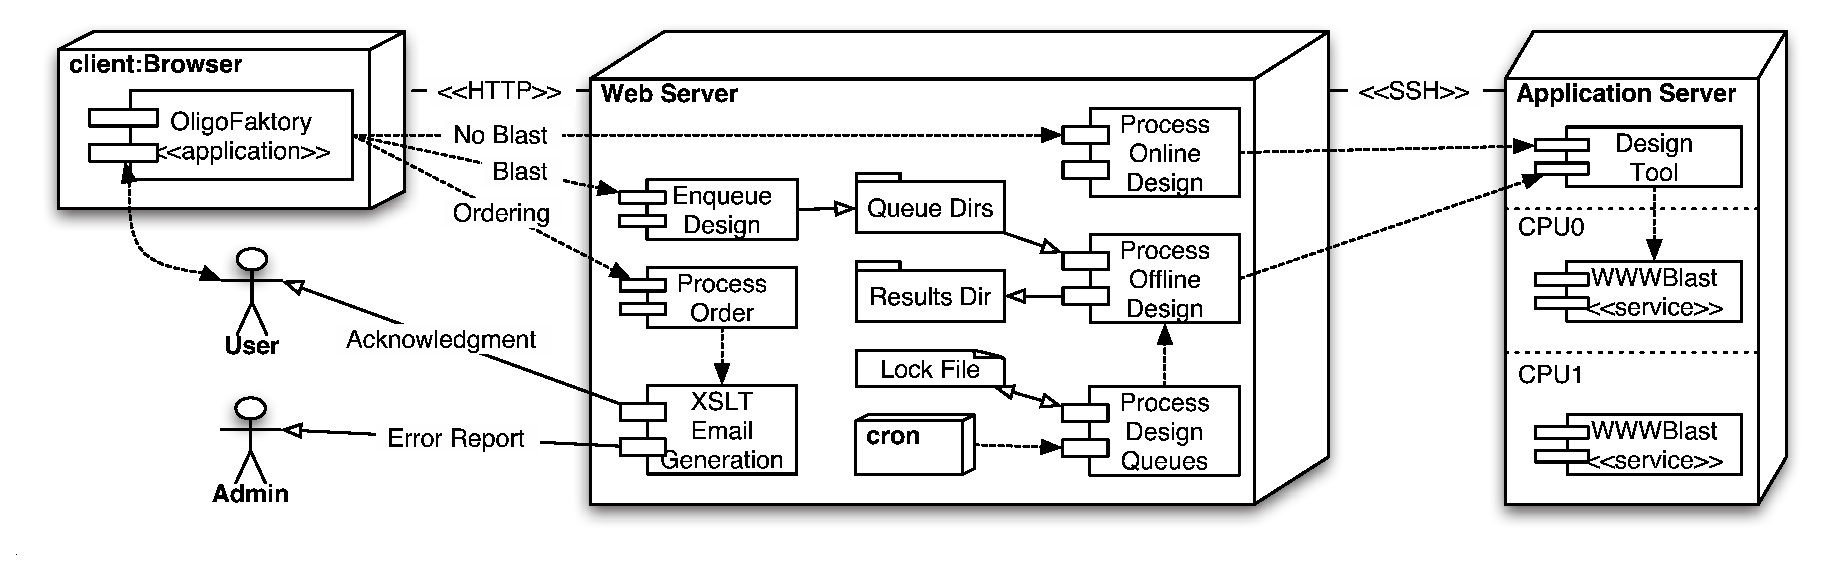
\includegraphics[width=12cm]{deployment_final.eps.eps}
% \caption{Deployment diagram of the queuing system behind the OligoFaktory web-portal. Filled arrows \includegraphics[height=1cm]{deployment_dependency_arrows.eps} represent dependencies, whereas \includegraphics{deployment_read_arrowS.eps} indicate read and/or write processes.}
\end{center}



\subsection*{Job Submission}

To submit a job, one just needs to create a file in a conventional queue directory. For our application, the file is the XML input for a design application, or an order to process. However, we could consider any executable files, like complex shell scripts \footnote{In this case, the queuing system should take the identity of the file's owner before executing it.}.

In our case, the directory structure for queues look like:

\begin{verbatim}
/var/lib/wwwrun/queues/
   ./order/
   ./longoligo/
   ./optiamp/
   ./sirna/
   ./analysis/
\end{verbatim}

When an application is running behind the queuing system, a lock file is created as a flag. This file does not exists while the system is idle. Results of designs applications are copied in:

\begin{verbatim}
/var/lib/wwwrun/results/
\end{verbatim}

Moreover, results or error reports will be sent by mail to users.

%%%%%%%%%%%%%%%%%%%%%%%%%%%%%%%%%%%%%%%%%%%%%%%%%%%%%%%%%%%%%%%%%%%%%%%%%%%%%%%%%%%%%%%%%%%%%%%%%%%%%

\subsection*{Job Watcher}

A crontab daemon periodically checks if files are stored in the queue directories. %This active loop process is similar to the one we could use to check for new e-mails.

The \texttt{crontab} file, \textbf{executes} the \texttt{process\_design\_queues.sh} and \texttt{process\_order\_queue.sh} scripts at given times or time intervals.

\begin{verbatim}
MAILTO=""
0 6, 12, 17 * * * /var/lib/wwwrun/process_order_queue.sh
* * * * * /var/lib/wwwrun/process_design_queues.sh \
optiamp longoligo analysis sirna
\end{verbatim}

In this example, ordering jobs are performed at 6:00, 12:00 and 17:00 each day. Design queries will be detected in less than a minute.

%%%%%%%%%%%%%%%%%%%%%%%%%%%%%%%%%%%%%%%%%%%%%%%%%%%%%%%%%%%%%%%%%%%%%%%%%%%%%%%%%%%%%%%%%%%%%%%%%%%%%

\subsection*{Offline Design Job Launcher}

The core of the system relies in the scripts launched by the cron daemon. These scripts will check if the resources are available, for instance by looking for the presence of a lock file. Several jobs could be executed in parallel, if we allow more than one lock file. However, for a computation intensive \noun{Blast} query, we chose to limite one job at a time.

The \texttt{process\_design\_queues.sh} script will 
\begin{enumerate}
	\item check if ressources are available, 
	\item lock the system and 
	\item for each xml file (\textit{.i.e} each job waiting to be run), \textbf{call} \texttt{process\_offline\_design.sh} with the appropriate parameters.
\end{enumerate}

\lstinputlisting[caption=process\_design\_queues.sh]{./scripts/process_design_queues.sh}
\bigskip

The \texttt{process\_offline\_design.sh} script 
\begin{enumerate}
	\item sets variables (like file names, email addresses...) and
	\item launches the computation over \texttt{ssh} on the application server
	\item notifies the user that the job is done or the user and the administrator that an error occured.
\end{enumerate}

\lstinputlisting[caption=process\_offline\_design.sh]{./scripts/process_offline_design.sh}
\bigskip

%%%%%%%%%%%%%%%%%%%%%%%%%%%%%%%%%%%%%%%%%%%%%%%%%%%%%%%%%%%%%%%%%%%%%%%%%%%%%%%%%%%%%%%%%%%%%%%%%%%%%

\subsection*{Online Design Job Launcher}

We provide the opportunity to directly run a design, independently of the queuing management. This is particularly useful when the web server wants to process a query file during an interactive user's session. Therefore, a waiting splash screen will be drawn during the design and the user will not receive any notification in his mailbox. 

The \texttt{process\_online\_design.sh} script performis similar tasks than \texttt{process\_offline\_design.sh} except that all output is displayed on the users screen.


\lstinputlisting[caption=process\_online\_design.sh]{./scripts/process_online_design.sh}
\bigskip

%%%%%%%%%%%%%%%%%%%%%%%%%%%%%%%%%%%%%%%%%%%%%%%%%%%%%%%%%%%%%%%%%%%%%%%%%%%%%%%%%%%%%%%%%%%%%%%%%%%%%

\subsection*{Order Job Launcher}

The ordering service yields the development of a supplementary script. Ideally, the third party facility should GET the orders from queue and process the available files, when they want and like they want. However, for technical and human reasons, we developed a PUT procedure. Periodically, we process orders, and sent two formated e-mails:

\begin{enumerate}
	\item A formated e-mail is sent to the ordering facility to launch effective synthesis.
	\item A human readable confirmation e-mail is sent to the customer. 
\end{enumerate}

The \texttt{process\_order\_queue.sh} program  (\textbf{called by} \texttt{crontab}) \textbf{runs} \texttt{results\_to\_customer.xsl} and \texttt{results\_to\_isogen.xsl} that make use of two XSL style-sheet to generate the content of these two e-mails.

\lstinputlisting[caption=process\_order\_queue.sh]{./scripts/process_order_queue.sh}
\bigskip

The \texttt{results\_to\_production.xsl} script will notify the ordering facility to launch effective synthesis.

\begin{small}
\lstset{language=xslt}
\lstinputlisting[caption=results\_to\_production.xsl]{./scripts/results_to_production.xsl}
\bigskip
\end{small}

The \texttt{results\_to\_customer.xsl} script will notify the custommer that the order has effectively been send.

\begin{small}
\lstinputlisting[caption=results\_to\_customer.xsl]{./scripts/results_to_customer.xsl}
\bigskip
\end{small}

%%%%%%%%%%%%%%%%%%%%%%%%%%%%%%%%%%%%%%%%%%%%%%%%%%%%%%%%%%%%%%%%%%%%%%%%%%%%%%%%%%%%%%%%%%%%%%%%%%%%%
%%%%%%%%%%%%%%%%%%%%%%%%%%%%%%%%%%%%%%%%%%%%%%%%%%%%%%%%%%%%%%%%%%%%%%%%%%%%%%%%%%%%%%%%%%%%%%%%%%%%%

\section*{Conclusions}

We described a lightweight solution to the implementation of a queuing system on UNIX systems. The described framework has been successfully implemented as a primer design portal (\url{http://ueg.ulb.ac.be/oligofaktory}) able to launch and manage several design applications.

\end{document}



